% Options for packages loaded elsewhere
\PassOptionsToPackage{unicode}{hyperref}
\PassOptionsToPackage{hyphens}{url}
%
\documentclass[
]{article}
\usepackage{lmodern}
\usepackage{amssymb,amsmath}
\usepackage{ifxetex,ifluatex}
\ifnum 0\ifxetex 1\fi\ifluatex 1\fi=0 % if pdftex
  \usepackage[T1]{fontenc}
  \usepackage[utf8]{inputenc}
  \usepackage{textcomp} % provide euro and other symbols
\else % if luatex or xetex
  \usepackage{unicode-math}
  \defaultfontfeatures{Scale=MatchLowercase}
  \defaultfontfeatures[\rmfamily]{Ligatures=TeX,Scale=1}
\fi
% Use upquote if available, for straight quotes in verbatim environments
\IfFileExists{upquote.sty}{\usepackage{upquote}}{}
\IfFileExists{microtype.sty}{% use microtype if available
  \usepackage[]{microtype}
  \UseMicrotypeSet[protrusion]{basicmath} % disable protrusion for tt fonts
}{}
\makeatletter
\@ifundefined{KOMAClassName}{% if non-KOMA class
  \IfFileExists{parskip.sty}{%
    \usepackage{parskip}
  }{% else
    \setlength{\parindent}{0pt}
    \setlength{\parskip}{6pt plus 2pt minus 1pt}}
}{% if KOMA class
  \KOMAoptions{parskip=half}}
\makeatother
\usepackage{xcolor}
\IfFileExists{xurl.sty}{\usepackage{xurl}}{} % add URL line breaks if available
\IfFileExists{bookmark.sty}{\usepackage{bookmark}}{\usepackage{hyperref}}
\hypersetup{
  pdftitle={STAT 33B Homework 1},
  pdfauthor={Ming Fong (3035619833)},
  hidelinks,
  pdfcreator={LaTeX via pandoc}}
\urlstyle{same} % disable monospaced font for URLs
\usepackage[margin=1in]{geometry}
\usepackage{color}
\usepackage{fancyvrb}
\newcommand{\VerbBar}{|}
\newcommand{\VERB}{\Verb[commandchars=\\\{\}]}
\DefineVerbatimEnvironment{Highlighting}{Verbatim}{commandchars=\\\{\}}
% Add ',fontsize=\small' for more characters per line
\usepackage{framed}
\definecolor{shadecolor}{RGB}{248,248,248}
\newenvironment{Shaded}{\begin{snugshade}}{\end{snugshade}}
\newcommand{\AlertTok}[1]{\textcolor[rgb]{0.94,0.16,0.16}{#1}}
\newcommand{\AnnotationTok}[1]{\textcolor[rgb]{0.56,0.35,0.01}{\textbf{\textit{#1}}}}
\newcommand{\AttributeTok}[1]{\textcolor[rgb]{0.77,0.63,0.00}{#1}}
\newcommand{\BaseNTok}[1]{\textcolor[rgb]{0.00,0.00,0.81}{#1}}
\newcommand{\BuiltInTok}[1]{#1}
\newcommand{\CharTok}[1]{\textcolor[rgb]{0.31,0.60,0.02}{#1}}
\newcommand{\CommentTok}[1]{\textcolor[rgb]{0.56,0.35,0.01}{\textit{#1}}}
\newcommand{\CommentVarTok}[1]{\textcolor[rgb]{0.56,0.35,0.01}{\textbf{\textit{#1}}}}
\newcommand{\ConstantTok}[1]{\textcolor[rgb]{0.00,0.00,0.00}{#1}}
\newcommand{\ControlFlowTok}[1]{\textcolor[rgb]{0.13,0.29,0.53}{\textbf{#1}}}
\newcommand{\DataTypeTok}[1]{\textcolor[rgb]{0.13,0.29,0.53}{#1}}
\newcommand{\DecValTok}[1]{\textcolor[rgb]{0.00,0.00,0.81}{#1}}
\newcommand{\DocumentationTok}[1]{\textcolor[rgb]{0.56,0.35,0.01}{\textbf{\textit{#1}}}}
\newcommand{\ErrorTok}[1]{\textcolor[rgb]{0.64,0.00,0.00}{\textbf{#1}}}
\newcommand{\ExtensionTok}[1]{#1}
\newcommand{\FloatTok}[1]{\textcolor[rgb]{0.00,0.00,0.81}{#1}}
\newcommand{\FunctionTok}[1]{\textcolor[rgb]{0.00,0.00,0.00}{#1}}
\newcommand{\ImportTok}[1]{#1}
\newcommand{\InformationTok}[1]{\textcolor[rgb]{0.56,0.35,0.01}{\textbf{\textit{#1}}}}
\newcommand{\KeywordTok}[1]{\textcolor[rgb]{0.13,0.29,0.53}{\textbf{#1}}}
\newcommand{\NormalTok}[1]{#1}
\newcommand{\OperatorTok}[1]{\textcolor[rgb]{0.81,0.36,0.00}{\textbf{#1}}}
\newcommand{\OtherTok}[1]{\textcolor[rgb]{0.56,0.35,0.01}{#1}}
\newcommand{\PreprocessorTok}[1]{\textcolor[rgb]{0.56,0.35,0.01}{\textit{#1}}}
\newcommand{\RegionMarkerTok}[1]{#1}
\newcommand{\SpecialCharTok}[1]{\textcolor[rgb]{0.00,0.00,0.00}{#1}}
\newcommand{\SpecialStringTok}[1]{\textcolor[rgb]{0.31,0.60,0.02}{#1}}
\newcommand{\StringTok}[1]{\textcolor[rgb]{0.31,0.60,0.02}{#1}}
\newcommand{\VariableTok}[1]{\textcolor[rgb]{0.00,0.00,0.00}{#1}}
\newcommand{\VerbatimStringTok}[1]{\textcolor[rgb]{0.31,0.60,0.02}{#1}}
\newcommand{\WarningTok}[1]{\textcolor[rgb]{0.56,0.35,0.01}{\textbf{\textit{#1}}}}
\usepackage{longtable,booktabs}
% Correct order of tables after \paragraph or \subparagraph
\usepackage{etoolbox}
\makeatletter
\patchcmd\longtable{\par}{\if@noskipsec\mbox{}\fi\par}{}{}
\makeatother
% Allow footnotes in longtable head/foot
\IfFileExists{footnotehyper.sty}{\usepackage{footnotehyper}}{\usepackage{footnote}}
\makesavenoteenv{longtable}
\usepackage{graphicx}
\makeatletter
\def\maxwidth{\ifdim\Gin@nat@width>\linewidth\linewidth\else\Gin@nat@width\fi}
\def\maxheight{\ifdim\Gin@nat@height>\textheight\textheight\else\Gin@nat@height\fi}
\makeatother
% Scale images if necessary, so that they will not overflow the page
% margins by default, and it is still possible to overwrite the defaults
% using explicit options in \includegraphics[width, height, ...]{}
\setkeys{Gin}{width=\maxwidth,height=\maxheight,keepaspectratio}
% Set default figure placement to htbp
\makeatletter
\def\fps@figure{htbp}
\makeatother
\setlength{\emergencystretch}{3em} % prevent overfull lines
\providecommand{\tightlist}{%
  \setlength{\itemsep}{0pt}\setlength{\parskip}{0pt}}
\setcounter{secnumdepth}{-\maxdimen} % remove section numbering
\ifluatex
  \usepackage{selnolig}  % disable illegal ligatures
\fi

\title{STAT 33B Homework 1}
\author{Ming Fong (3035619833)}
\date{Sep 10, 2020}

\begin{document}
\maketitle

This homework is due \textbf{Sep 10, 2020} by 11:59pm PT.

Homeworks are graded for correctness.

As you work, write your answers in this notebook. Answer questions with
complete sentences, and put code in code chunks. You can make as many
new code chunks as you like.

Please do not delete the exercises already in this notebook, because it
may interfere with our grading tools.

You need to submit your work in two places:

\begin{itemize}
\tightlist
\item
  Submit this Rmd file with your edits on bCourses.
\item
  Knit and submit the generated PDF file on Gradescope.
\end{itemize}

\hypertarget{exercise-1}{%
\subsection{Exercise 1}\label{exercise-1}}

Note: In R Markdown formatting, a dollar sign \texttt{\$} marks the
beginning of a (LaTeX) mathematical expression. For example, to format a
linear equation nicely, you can write \(ax + b = 0\). You don't need to
know LaTeX for this class, so if you don't understand something written
inside \texttt{\$}, knit the PDF and read that instead.

The \texttt{curve()} function plots a curve based on an expression. The
basic syntax is \texttt{curve(expr,\ from,\ to)} where \texttt{from} and
\texttt{to} are the limits of the x-axis.

For example, to plot \(x^2\) between 0 and 3:

\begin{Shaded}
\begin{Highlighting}[]
\KeywordTok{curve}\NormalTok{(x}\OperatorTok{\^{}}\DecValTok{2}\NormalTok{, }\DecValTok{0}\NormalTok{, }\DecValTok{3}\NormalTok{)}
\end{Highlighting}
\end{Shaded}

\includegraphics{hw1_files/figure-latex/unnamed-chunk-1-1.pdf}

The \texttt{curve()} function makes it possible to use R as a graphing
calculator.

For each expression below:

\begin{enumerate}
\def\labelenumi{\arabic{enumi}.}
\item
  Plot the expression so that all points where it is 0 are visible.
  Experiment to find appropriate limits for the x-axis.
\item
  At which point(s) is the expression zero? Estimate (within 1 unit)
  based on your plot rather than computing these mathematically.
\end{enumerate}

Here are the expressions:

\begin{enumerate}
\def\labelenumi{\arabic{enumi}.}
\tightlist
\item
  \(5x - 1\)
\item
  \(3x^2 - 2x - 8\)
\item
  \(\sqrt{3x} - 4\)
\end{enumerate}

\hypertarget{your-answer-goes-here}{%
\subsubsection{YOUR ANSWER GOES HERE:}\label{your-answer-goes-here}}

\begin{enumerate}
\def\labelenumi{\arabic{enumi}.}
\tightlist
\item
  Zero at approximately \(x = 0.2\)
\end{enumerate}

\begin{Shaded}
\begin{Highlighting}[]
\KeywordTok{curve}\NormalTok{(}\DecValTok{5}\OperatorTok{*}\NormalTok{x }\OperatorTok{{-}}\StringTok{ }\DecValTok{1}\NormalTok{, }\DecValTok{0}\NormalTok{, }\DecValTok{2}\NormalTok{)}
\end{Highlighting}
\end{Shaded}

\includegraphics{hw1_files/figure-latex/unnamed-chunk-2-1.pdf}

\begin{enumerate}
\def\labelenumi{\arabic{enumi}.}
\setcounter{enumi}{1}
\tightlist
\item
  Zeros at approximately \(x = -1.5, 2\)
\end{enumerate}

\begin{Shaded}
\begin{Highlighting}[]
\KeywordTok{curve}\NormalTok{(}\DecValTok{3}\OperatorTok{*}\NormalTok{x}\OperatorTok{\^{}}\DecValTok{2} \OperatorTok{{-}}\StringTok{ }\DecValTok{2}\OperatorTok{*}\NormalTok{x }\OperatorTok{{-}}\StringTok{ }\DecValTok{8}\NormalTok{, }\DecValTok{{-}5}\NormalTok{, }\DecValTok{5}\NormalTok{)}
\end{Highlighting}
\end{Shaded}

\includegraphics{hw1_files/figure-latex/unnamed-chunk-3-1.pdf}

\begin{enumerate}
\def\labelenumi{\arabic{enumi}.}
\setcounter{enumi}{2}
\tightlist
\item
  Zero at approximately \(x = 0\)
\end{enumerate}

\begin{Shaded}
\begin{Highlighting}[]
\KeywordTok{curve}\NormalTok{(}\KeywordTok{sqrt}\NormalTok{(}\DecValTok{3}\OperatorTok{*}\NormalTok{x), }\DecValTok{0}\NormalTok{, }\DecValTok{5}\NormalTok{)}
\end{Highlighting}
\end{Shaded}

\includegraphics{hw1_files/figure-latex/unnamed-chunk-4-1.pdf}

\hypertarget{exercise-2}{%
\subsection{Exercise 2}\label{exercise-2}}

A \textbf{discrete probability distribution} is a table of mutually
exclusive outcomes and their associated probabilities.

For example, the \textbf{discrete uniform distribution} assigns equal
probability to each outcome. So the discrete uniform distribution on the
integers 1-4 is:

\begin{longtable}[]{@{}ll@{}}
\toprule
Outcome & Probability\tabularnewline
\midrule
\endhead
1 & 0.25\tabularnewline
2 & 0.25\tabularnewline
3 & 0.25\tabularnewline
4 & 0.25\tabularnewline
\bottomrule
\end{longtable}

A fair coin toss is another instance of a discrete uniform distribution,
where each of the two outcomes has probability 0.5.

You can plot the distribution above with the code:

\begin{Shaded}
\begin{Highlighting}[]
\NormalTok{outcome =}\StringTok{ }\KeywordTok{seq}\NormalTok{(}\DecValTok{1}\NormalTok{, }\DecValTok{4}\NormalTok{)}
\NormalTok{prob =}\StringTok{ }\KeywordTok{rep}\NormalTok{(}\FloatTok{0.25}\NormalTok{, }\DecValTok{4}\NormalTok{)}
\KeywordTok{plot}\NormalTok{(outcome, prob)}
\end{Highlighting}
\end{Shaded}

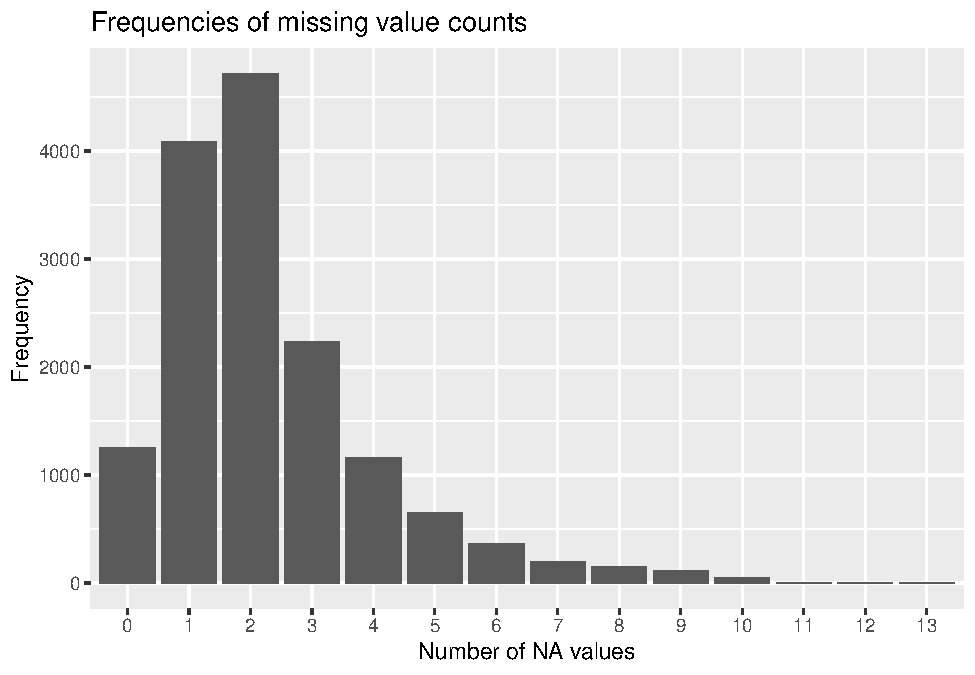
\includegraphics{hw1_files/figure-latex/unnamed-chunk-5-1.pdf}

Because the probabilities are all equal, a plot of a uniform
distribution is always flat, regardless of the number of outcomes.

The idea of a uniform distribution can also be extended to continuous
values. For example, suppose we want to select a decimal value between 0
and 4 (inclusive), with equal probability for any value in the interval.
This is a \textbf{countinuous uniform distribution}.

As with any uniform distribution, a plot of a continuous uniform
distribution is flat. However, instead of discrete points, the
distribution is a curve along an interval.

You can plot the continuous uniform distribution from 0 to 4 with the
code:

\begin{Shaded}
\begin{Highlighting}[]
\KeywordTok{curve}\NormalTok{(}\KeywordTok{dunif}\NormalTok{(x, }\DecValTok{0}\NormalTok{, }\DecValTok{4}\NormalTok{), }\DecValTok{{-}1}\NormalTok{, }\DecValTok{5}\NormalTok{, }\DataTypeTok{n =} \DecValTok{1000}\NormalTok{)}
\end{Highlighting}
\end{Shaded}

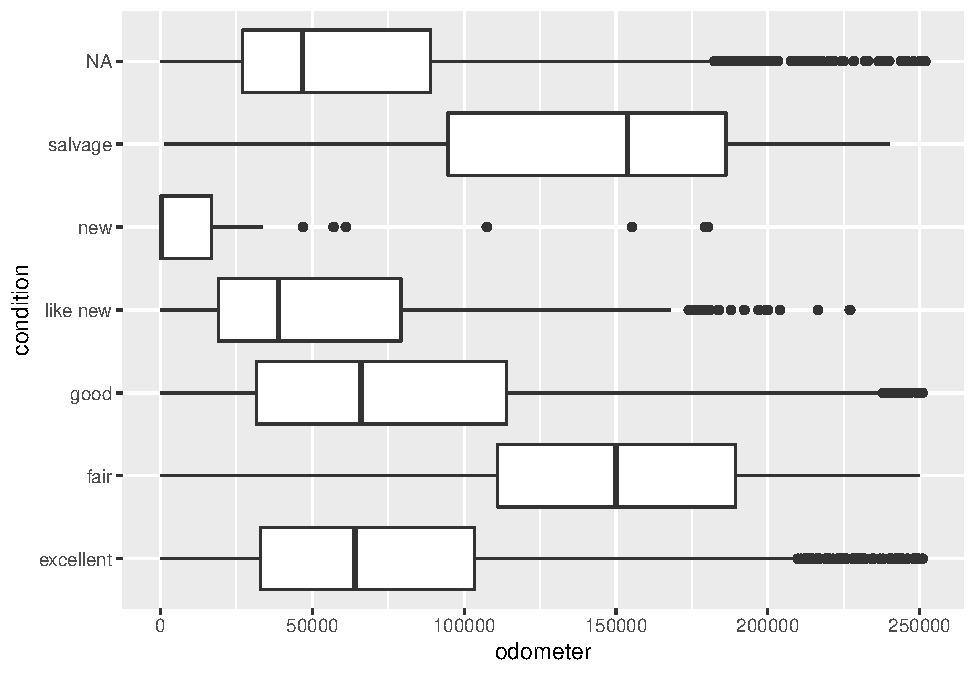
\includegraphics{hw1_files/figure-latex/unnamed-chunk-6-1.pdf}

A plot of a continuous distribution is called a \textbf{density plot}.

In a density plot, the y-axis no longer represents probability. Instead,
the probability of points in any subinterval is the total area between
the curve and the line \(y = 0\) over the subinterval. For instance, in
the distribution above, the probability of the outcome being a point
between 1 and 2 (inclusive) is 0.25.

R provides functions to compute the density of various distributions.
The code above uses the \texttt{dunif()} function, the \textbf{d}ensity
plot function for the \textbf{unif}orm distribution. The function has
parameters to control the interval for the distribution.

R also provides functions to sample values randomly from various
distributions. For example, the \texttt{runif()} function samples
\textbf{r}andomly from a continuous \textbf{unif}orm distribution. You
can sample 10 values from the continuous uniform distribution from -1 to
1 with the code:

\begin{Shaded}
\begin{Highlighting}[]
\KeywordTok{runif}\NormalTok{(}\DecValTok{10}\NormalTok{, }\DecValTok{{-}1}\NormalTok{, }\DecValTok{1}\NormalTok{)}
\end{Highlighting}
\end{Shaded}

\begin{verbatim}
##  [1] -0.8180239  0.7108587 -0.9457545  0.2886718 -0.6005458 -0.3572614
##  [7]  0.9046318  0.2254425  0.8532265 -0.7445967
\end{verbatim}

Since these values are randomly sampled, they will be different each
time you run the code.

The \textbf{Gaussian distribution} or normal distribution is another
continuous probability distribution. The distribution plays an important
role in mathematics, statistics, and the natural sciences. The density
plot for this distribution is often described as a ``bell-shaped
curve''. The Gaussian distribution is typically parameterized by its
mean (center) and standard deviation (how spread out it is), rather than
the interval it covers.

R provides functions \texttt{dnorm()} and \texttt{rnorm()} for the
Gaussian distribution that are analogous to the \texttt{dunif()} and
\texttt{runif()} functions described above.

\begin{enumerate}
\def\labelenumi{\arabic{enumi}.}
\item
  Use the \texttt{curve()} function to make a density plot of the
  Gaussian distribution with mean 10 and standard deviation 5. Set the
  x-axis to span from -10 to 30.
\item
  Skim the documentation for \texttt{rnorm()}. Then create a variable
  called \texttt{samp} that contains 10 random values from a normal
  distribution with mean 10 and standard deviation 5.
\item
  Compute the mean and standard deviation of \texttt{samp}. Comment
  briefly on how much these differ from the true mean 10 and true
  standard deviation 5.

  What happens if you run your code a second time? Are the sample mean
  and standard deviation the same? Are the sampled points the same?
\end{enumerate}

\hypertarget{your-answer-goes-here-1}{%
\subsubsection{YOUR ANSWER GOES HERE:}\label{your-answer-goes-here-1}}

\begin{enumerate}
\def\labelenumi{\arabic{enumi}.}
\tightlist
\item
\end{enumerate}

\begin{Shaded}
\begin{Highlighting}[]
\KeywordTok{curve}\NormalTok{(}\KeywordTok{dnorm}\NormalTok{(x, }\DecValTok{10}\NormalTok{, }\DecValTok{5}\NormalTok{), }\DecValTok{{-}10}\NormalTok{, }\DecValTok{30}\NormalTok{)}
\end{Highlighting}
\end{Shaded}

\includegraphics{hw1_files/figure-latex/unnamed-chunk-8-1.pdf}

\begin{enumerate}
\def\labelenumi{\arabic{enumi}.}
\setcounter{enumi}{1}
\tightlist
\item
\end{enumerate}

\begin{Shaded}
\begin{Highlighting}[]
\NormalTok{mu =}\StringTok{ }\DecValTok{10}
\NormalTok{sigma =}\StringTok{ }\DecValTok{5}
\NormalTok{samp =}\StringTok{ }\KeywordTok{rnorm}\NormalTok{(}\DecValTok{10}\NormalTok{, mu, sigma)}
\NormalTok{samp}
\end{Highlighting}
\end{Shaded}

\begin{verbatim}
##  [1] 13.339538  1.589604 18.172134 10.581736 11.856612  7.739454  2.349451
##  [8]  8.188245  5.608598 16.492769
\end{verbatim}

\begin{enumerate}
\def\labelenumi{\arabic{enumi}.}
\setcounter{enumi}{2}
\tightlist
\item
  Running the code many times will change the random sample and also
  change the sample mean and sd. The difference is computed below.
\end{enumerate}

\begin{Shaded}
\begin{Highlighting}[]
\NormalTok{mu2 =}\StringTok{ }\KeywordTok{mean}\NormalTok{(samp)}
\NormalTok{mu2}
\end{Highlighting}
\end{Shaded}

\begin{verbatim}
## [1] 9.591814
\end{verbatim}

\begin{Shaded}
\begin{Highlighting}[]
\CommentTok{\# The mean of the sample differs from the orignal mean by}
\NormalTok{mu2 }\OperatorTok{{-}}\StringTok{ }\NormalTok{mu}
\end{Highlighting}
\end{Shaded}

\begin{verbatim}
## [1] -0.4081859
\end{verbatim}

\begin{Shaded}
\begin{Highlighting}[]
\NormalTok{sigma2 =}\StringTok{ }\KeywordTok{sd}\NormalTok{(samp)}
\NormalTok{sigma2}
\end{Highlighting}
\end{Shaded}

\begin{verbatim}
## [1] 5.569303
\end{verbatim}

\begin{Shaded}
\begin{Highlighting}[]
\CommentTok{\# The standard deviation of the sample differs from the orignal standard deviation by}
\NormalTok{sigma2 }\OperatorTok{{-}}\StringTok{ }\NormalTok{sigma}
\end{Highlighting}
\end{Shaded}

\begin{verbatim}
## [1] 0.5693029
\end{verbatim}

\hypertarget{exercise-3}{%
\subsection{Exercise 3}\label{exercise-3}}

R's functions for random sampling use a pseudo-random number generator
(PRNG). The numbers produced by a PRNG are not truly random, but satisfy
conditions that make them close enough to random for most scientific
computing tasks.

An advantage of PRNGs is that they are deterministic. Given the same
initial parameter, called a \textbf{seed}, a PRNG will generate the same
sequence of ``random'' numbers every time. When you start R, the seed is
automatically assigned value from your computer that varies (e.g., the
system time in milliseconds). This ensures that you get a different
sequence of random numbers in each R session.

You can the PRNG seed with the \texttt{set.seed()} function. Setting the
seed makes your results reproducible. That is, other people can run your
code and get the same results even if the code generates random numbers.

Generally, you should only set the seed once at the beginning of an R
script or notebook, because it affects all subsequent calls that use the
PRNG.

\begin{enumerate}
\def\labelenumi{\arabic{enumi}.}
\item
  Set the seed to 93.
\item
  Create a variable called \texttt{samp} that contains 1000 random
  values from a normal distribution with mean 10 and standard deviation
  5.
\item
  Compute the mean and standard deviation of \texttt{samp}.

  What happens if you run your code a second time? Are the sample mean
  and standard deviation the same? Are the sampled points the same?
  Explain how step 1 affects this.
\item
  Compute the number of values in \texttt{samp} that are greater than 8.
  \emph{Hint: there is a fast, simple way to count \texttt{TRUE} values
  using implicit coercion.}
\end{enumerate}

\hypertarget{your-answer-goes-here-2}{%
\subsubsection{YOUR ANSWER GOES HERE:}\label{your-answer-goes-here-2}}

\begin{enumerate}
\def\labelenumi{\arabic{enumi}.}
\tightlist
\item
\end{enumerate}

\begin{Shaded}
\begin{Highlighting}[]
\KeywordTok{set.seed}\NormalTok{(}\DecValTok{93}\NormalTok{)}
\end{Highlighting}
\end{Shaded}

\begin{enumerate}
\def\labelenumi{\arabic{enumi}.}
\setcounter{enumi}{1}
\tightlist
\item
\end{enumerate}

\begin{Shaded}
\begin{Highlighting}[]
\NormalTok{samp =}\StringTok{ }\KeywordTok{rnorm}\NormalTok{(}\DecValTok{1000}\NormalTok{, }\DecValTok{10}\NormalTok{, }\DecValTok{5}\NormalTok{)}
\end{Highlighting}
\end{Shaded}

\begin{enumerate}
\def\labelenumi{\arabic{enumi}.}
\setcounter{enumi}{2}
\tightlist
\item
  If you set the seed and run the code again, the sampled points are
  always the same. \texttt{set.seed()} ensures the pseudo-random numbers
  used in \texttt{rnorm()} are the same each time.
\end{enumerate}

\begin{Shaded}
\begin{Highlighting}[]
\KeywordTok{mean}\NormalTok{(samp)}
\end{Highlighting}
\end{Shaded}

\begin{verbatim}
## [1] 10.1505
\end{verbatim}

\begin{Shaded}
\begin{Highlighting}[]
\KeywordTok{sd}\NormalTok{(samp)}
\end{Highlighting}
\end{Shaded}

\begin{verbatim}
## [1] 5.127733
\end{verbatim}

\begin{enumerate}
\def\labelenumi{\arabic{enumi}.}
\setcounter{enumi}{3}
\tightlist
\item
\end{enumerate}

\begin{Shaded}
\begin{Highlighting}[]
\KeywordTok{sum}\NormalTok{(samp }\OperatorTok{\textgreater{}}\StringTok{ }\DecValTok{8}\NormalTok{)}
\end{Highlighting}
\end{Shaded}

\begin{verbatim}
## [1] 668
\end{verbatim}

\hypertarget{exercise-4}{%
\subsection{Exercise 4}\label{exercise-4}}

A \textbf{Monte Carlo algorithm} is an algorithm that uses random number
generation to approximate a non-random result.

One application of Monte Carlo algorithms is to approximate the area of
a shape. In this exercise, you'll use a Monte Carlo algorithm to
approximate the area of a circle, and thereby approximate pi.

Consider the circle centered at 0 with radius 1. Points on the circle
satisfy \(x^2 + y^2 = 1\). This is the ``target shape'' for which you'll
approximate the area. In practice, the target shape is usually one whose
area is difficult to compute by hand.

In order to approximate the area of the target shape, start by finding a
square or rectangle that completely encloses the target shape. For
instance, we can use the square with corners (-1, -1) and (1, 1) to
enclose the circle.

Next, randomly sample x coordinates and y coordinates uniformly and
independently over the square.

Now the proportion of sampled points inside the circle corresponds to
the ratio between the area of the circle and the area of the square.
Since you know the area of the square, you can use this relationship to
compute the area of the circle.

\begin{enumerate}
\def\labelenumi{\arabic{enumi}.}
\item
  Use R and the described algorithm to approximate the value of pi. Use
  a variable called \texttt{n} to control the sample size.

  Do not use if-statements or loops in your solution; they are not
  necessary. Try to take advantage of vectorization and implicit
  coercion. A typical solution will be 2-6 lines.
\item
  Test your code for different values of \texttt{n} from 10 to
  1,000,000. How does changing \texttt{n} affect the accuracy of the
  approximation? How does it affect the time it takes to compute the
  approximation?

  \emph{Hint 1: R supports exponent notation, so you can write 1,000,000
  in R as \texttt{1e6}.}

  \emph{Hint 2: The \texttt{microbenchmark} package provides a simple
  function called \texttt{microbenchmark()} for timing expressions. You
  can use it to time an entire block of code by surrounding the code
  with curly braces \texttt{\{\ \}}.}
\end{enumerate}

\hypertarget{your-answer-goes-here-3}{%
\subsubsection{YOUR ANSWER GOES HERE:}\label{your-answer-goes-here-3}}

\begin{enumerate}
\def\labelenumi{\arabic{enumi}.}
\tightlist
\item
\end{enumerate}

\begin{Shaded}
\begin{Highlighting}[]
\NormalTok{monte\_carlo =}\StringTok{ }\ControlFlowTok{function}\NormalTok{(}\DataTypeTok{n =} \DecValTok{1000}\NormalTok{) \{}
\NormalTok{   x =}\StringTok{ }\KeywordTok{runif}\NormalTok{(n, }\DecValTok{{-}1}\NormalTok{, }\DecValTok{1}\NormalTok{)}
\NormalTok{   y =}\StringTok{ }\KeywordTok{runif}\NormalTok{(n, }\DecValTok{{-}1}\NormalTok{, }\DecValTok{1}\NormalTok{)}
\NormalTok{   (}\KeywordTok{sum}\NormalTok{(x}\OperatorTok{\^{}}\DecValTok{2} \OperatorTok{+}\StringTok{ }\NormalTok{y}\OperatorTok{\^{}}\DecValTok{2} \OperatorTok{\textless{}}\StringTok{ }\DecValTok{1}\NormalTok{) }\OperatorTok{/}\StringTok{ }\NormalTok{n) }\OperatorTok{*}\StringTok{ }\DecValTok{4}
\NormalTok{\}}
\KeywordTok{monte\_carlo}\NormalTok{()}
\end{Highlighting}
\end{Shaded}

\begin{verbatim}
## [1] 3.128
\end{verbatim}

\begin{enumerate}
\def\labelenumi{\arabic{enumi}.}
\setcounter{enumi}{1}
\tightlist
\item
\end{enumerate}

\begin{Shaded}
\begin{Highlighting}[]
\KeywordTok{library}\NormalTok{(microbenchmark)}
\KeywordTok{monte\_carlo}\NormalTok{(}\DecValTok{10}\NormalTok{)}
\end{Highlighting}
\end{Shaded}

\begin{verbatim}
## [1] 2.8
\end{verbatim}

\begin{Shaded}
\begin{Highlighting}[]
\KeywordTok{microbenchmark}\NormalTok{(}\KeywordTok{monte\_carlo}\NormalTok{(}\DecValTok{10}\NormalTok{))}
\end{Highlighting}
\end{Shaded}

\begin{verbatim}
## Unit: microseconds
##             expr   min    lq    mean median    uq    max neval
##  monte_carlo(10) 7.301 7.851 8.86804  8.201 8.751 54.302   100
\end{verbatim}

\begin{Shaded}
\begin{Highlighting}[]
\KeywordTok{monte\_carlo}\NormalTok{(}\DecValTok{100000}\NormalTok{)}
\end{Highlighting}
\end{Shaded}

\begin{verbatim}
## [1] 3.1378
\end{verbatim}

\begin{Shaded}
\begin{Highlighting}[]
\KeywordTok{microbenchmark}\NormalTok{(}\KeywordTok{monte\_carlo}\NormalTok{(}\DecValTok{100000}\NormalTok{))}
\end{Highlighting}
\end{Shaded}

\begin{verbatim}
## Unit: milliseconds
##                expr      min       lq     mean   median       uq     max neval
##  monte_carlo(1e+05) 7.389301 7.949001 8.657686 8.380501 8.874051 15.3774   100
\end{verbatim}

\begin{Shaded}
\begin{Highlighting}[]
\KeywordTok{monte\_carlo}\NormalTok{(}\DecValTok{1000000}\NormalTok{)}
\end{Highlighting}
\end{Shaded}

\begin{verbatim}
## [1] 3.141948
\end{verbatim}

\begin{Shaded}
\begin{Highlighting}[]
\KeywordTok{microbenchmark}\NormalTok{(}\KeywordTok{monte\_carlo}\NormalTok{(}\DecValTok{1000000}\NormalTok{))}
\end{Highlighting}
\end{Shaded}

\begin{verbatim}
## Unit: milliseconds
##                expr     min      lq    mean  median       uq      max neval
##  monte_carlo(1e+06) 77.4741 82.5979 86.2263 85.1192 88.50615 128.4792   100
\end{verbatim}

\end{document}
